\chapter{Analiza problemu}
\label{cha:Analiza probemu}

Rozpatrywanym problemem jest detekcja obiektów za pomocą sztucznej sieci neuronowej.
Realizacja zadania ma zostać przeprowadzona na wbudowanej platformie obliczeniowej typu SoC (ang. System on Chip).
W niniejszym rozdziale zostaną przedstawione założenia oraz wymagania stawiane wobec opracowywanego systemu detekcji.
Zostanie opisana docelowa platforma obliczeniowa. Zostaną przedstawione wybrane możliwe rozwiązania, 
a także dostępne narzędzia wspomagające docelową implementację.

% Opracowywany system powstaje na potrzeby konkursu \emph{Design Automation Conference System Design Contest 2021}. 
% Celem konkursu jest wykrycie pojedynczych obiektów na obrazach pochodzących z sekwencji zarejestrowanych podczas lotu dronem.


\section{Wymagania}
Ze względu, iż opracowywany system powstaje na potrzeby konkursu, 
musi on spełniać stawiane założenia i wymagania.
Zadaniem jest detekcja siecią neuronową pojedynczych obiektów w sekwencjach zarejestrowanych podczas lotu dronem.
Organizatorzy dostarczają zbiór treningowy składający się z obrazów o wymiarach 640 pikseli szerokości na 360 pikseli wysokości. Zbiór składa się z ponad 90 tysięcy obrazów, wchodzących w skład 95 sekwencji podzielonych na 12 kategorii. Na rysunku \ref{fig:sample_images} przedstawiono przykładowe obrazy znajdujące się w zbiorze uczącym wraz z zaznaczonymi obiektami detekcji. 

\begin{figure}
    \centering
    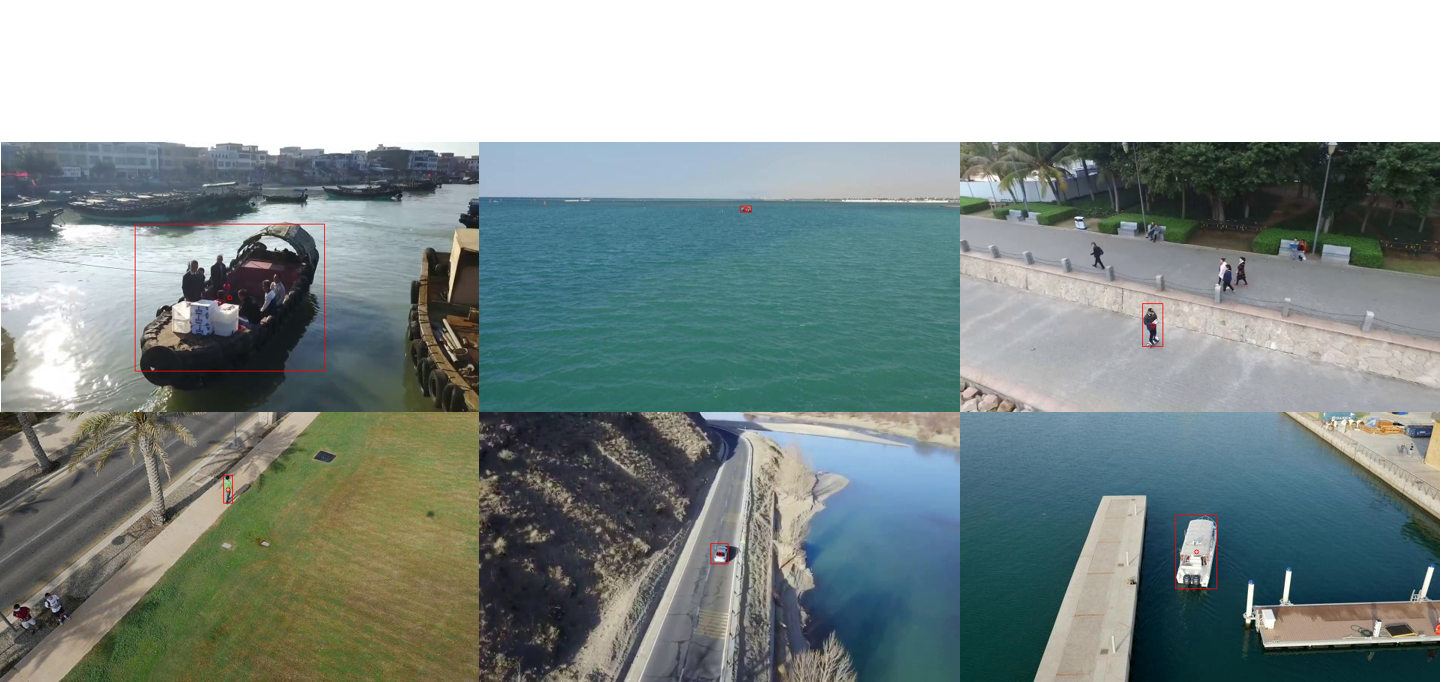
\includegraphics[width=\linewidth]{images/sample_images.png}
    \caption{Przykładowe obrazy zbioru uczącego wraz z zaznaczonymi obiektami detekcji.}
    \label{fig:sample_images}
\end{figure}

Wśród wymagań znajdują się również informacje odnośnie dostarczenia wymaganych plików.
Aplikacja sterująca ma być zrealizowana w postaci notatnika \emph{Jupyter}.
Dodatkowo należy dostarczyć również pliki \emph{*.hwh} (plik opisu diagramu blokowego logiki reprogramowalnej)
oraz \emph{*.bit} (plik konfiguracji części reprogramowalnej).

% - wymagania konkursu
% - wymagane pliki,
% - platforma(i jej opis) itp.

\section{Przegląd rozwiązań}
- analiza sieci YOLO z ultranet, SkyNet

- QNN i BNN

- (ten pod rozdział można by potraktować poniekąd jako przegląd literatury o sieciach/rozwiązaniach energooszczędnych)


\section{Narzędzia}
Przegląd narzędzi wspomagających implementację sprzętową:

- Vitis AI

- FINN + Brevitas

- hls4ml + QKeras


%---------------------------------------------------------------------------

    

